\section{Related Work}
\label{sec:related}

Answering the readiness question requires comparable field evidence for both
workload classes. Prior work provides interoperable messages, network and edge
procedures, systems for individual CAV applications, and measurements of direct
or network-assisted paths. Figure~\ref{fig:rw-gap} organizes these foundations
around the capabilities required for cooperative transportation. The primary
gap is a common application-level evaluation of compact CV/ITS updates and
correlated CAV operations over both path classes. Such an evaluation also needs
one application contract that represents the two workload classes consistently.

\begin{figure*}[!t]
  \centering
  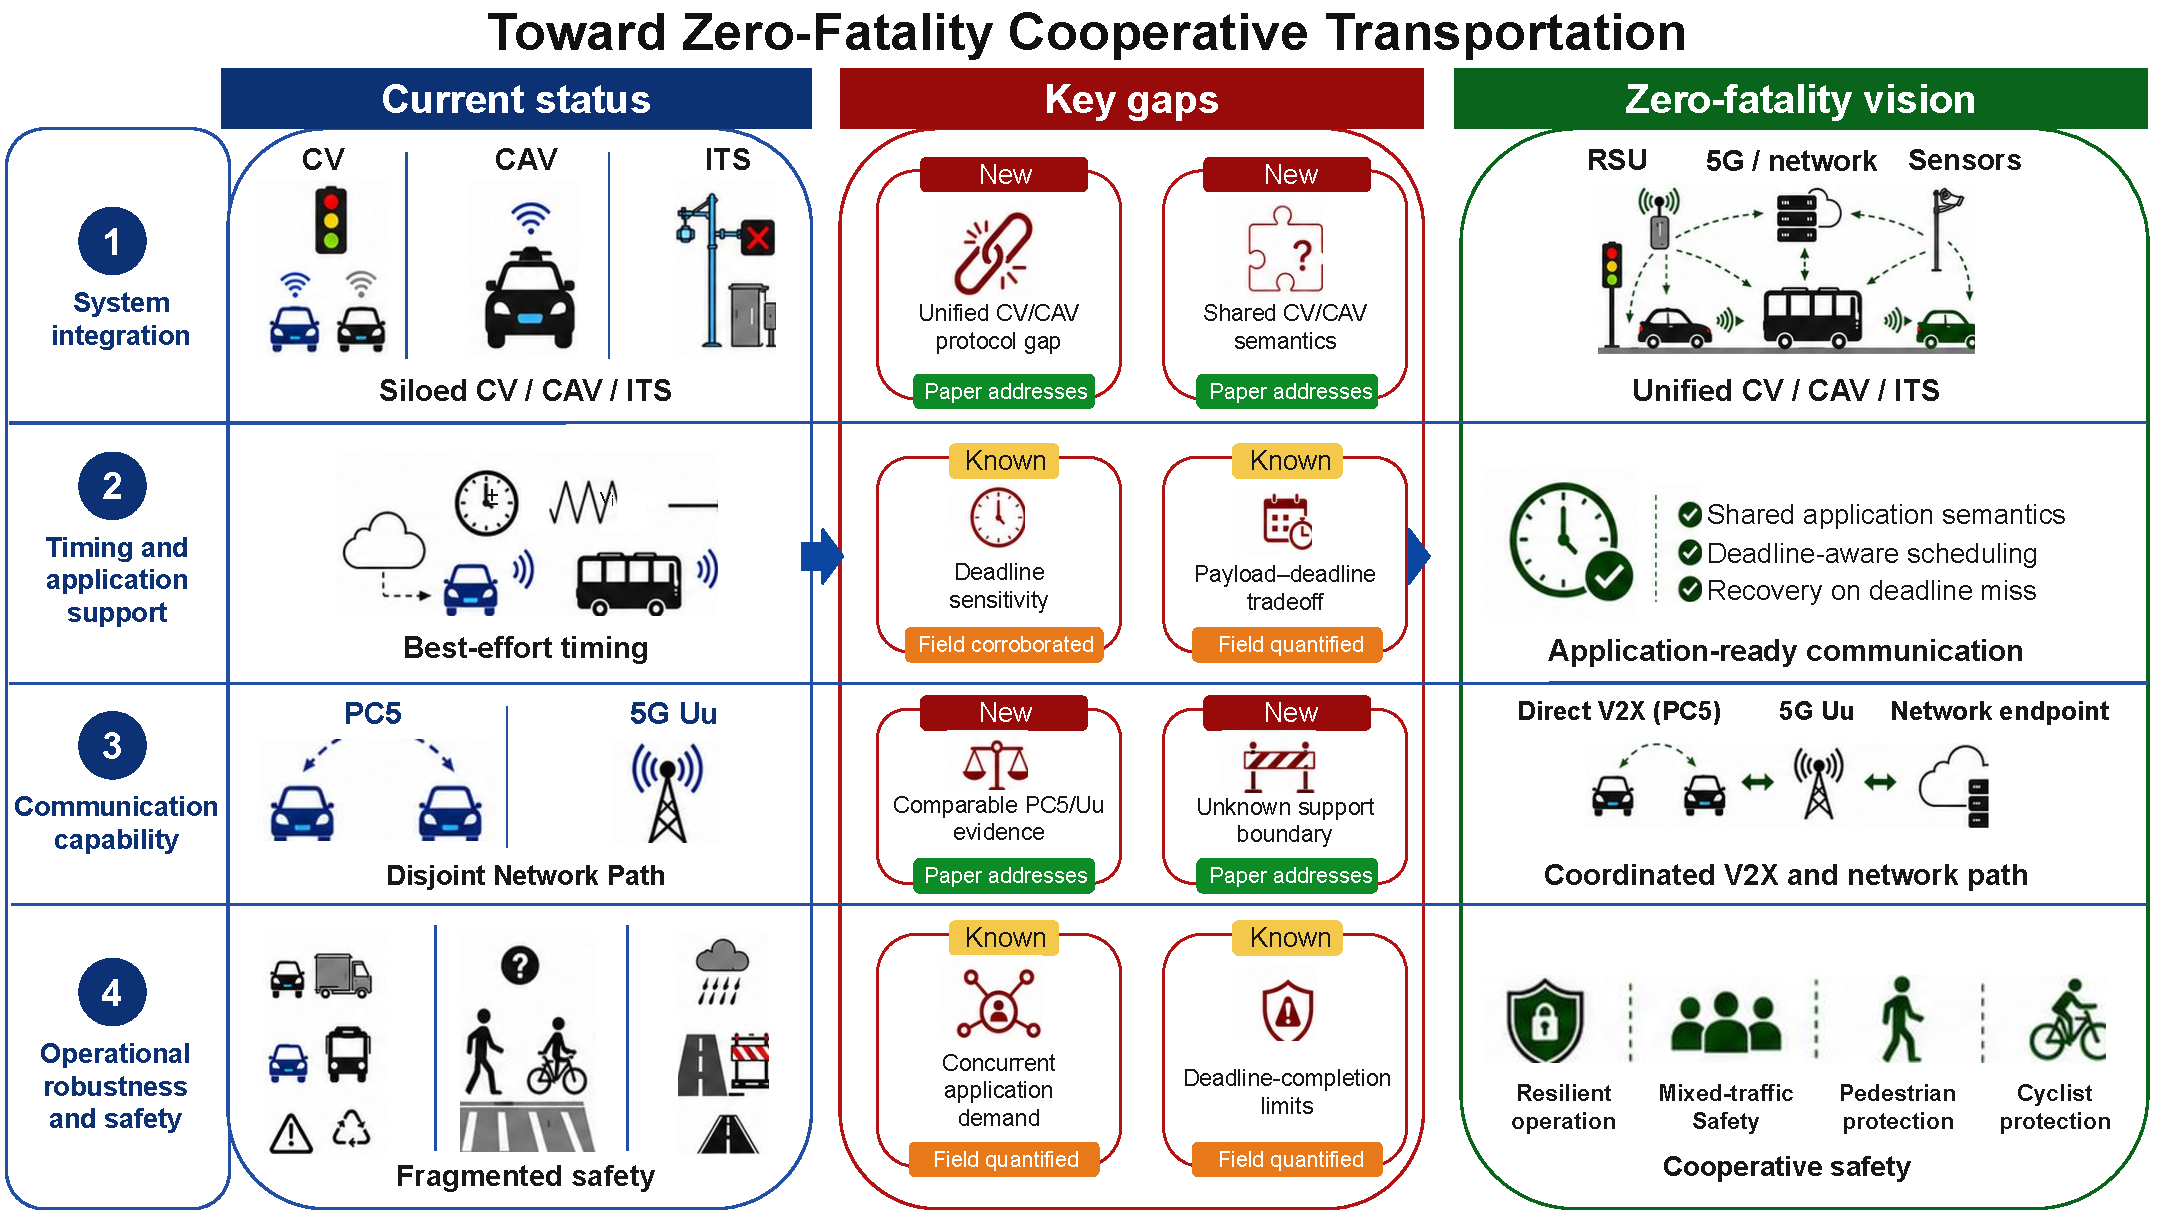
\includegraphics[width=\textwidth]{figs/figure01_related_work_landscape.pdf}
  \caption{Communication capabilities required for cooperative transportation.
  Existing technologies address individual message, application, and path
  functions. The measurement study determines when the two workload classes
  meet their application requirements, and IPI supplies the application
  contract used to represent them.}
  \Description{A three-column, four-row diagram connects current CV, CAV, and
  ITS communication to missing application integration and field evidence, then
  to future capabilities for deadline-aware communication, coordinated paths,
  and resilient cooperative safety.}
  \label{fig:rw-gap}
\end{figure*}

\textbf{Standards and application platforms.}
Vehicular interoperability is divided among application messages, network
services, and edge information exchange. SAE International J2735 defines safety, road-user,
map, signal, and priority messages for CV and ITS applications
\cite{saej2735_2020}. The Third Generation Partnership Project (3GPP) defines
PC5 and Uu communication and a V2X Application Enabler with registration,
delivery, resource-management, continuity, and session procedures
\cite{etsi123287r18,etsi123286r18}. The European Telecommunications Standards
Institute (ETSI) Multi-access Edge Computing (MEC) V2X Information Service adds
PC5/Uu provisioning, predicted quality of service, publication, and
subscription procedures \cite{etsimec030}. Architectures and platforms from
the 5G Automotive Association, ETSI, V2X Hub, and CARMA connect selected actors
and deployment functions
\cite{fivegaa2020architecture,etsi302665,usdotv2xhub,usdotcarma}.

Together, these mechanisms define complementary forms of interoperability.
J2735 defines individual application messages, 3GPP coordinates V2X application
services and sessions, and MEC distributes V2X information. We found no surveyed
implementation that combines byte-preserving J2735 carriage with generic,
correlated CAV operations behind one application contract for both PC5 and Uu.
The evaluation needs this combination to preserve workload meaning and operation
association as the communication path changes. IPI supplies the enabling
contract without replacing the message, service, or network standards beneath
it.

\textbf{CAV systems and middleware.}
Networked CAV systems demonstrate why application representation affects
communication demand. EMP and AutoCast select cooperative-perception
information \cite{zhang2021emp,qiu2022autocast}, while VIPS, VI-Map, and SOAR
return fused perception, compact maps, or coordinated infrastructure results
\cite{shi2022vips,he2023vimap,shi2024soar}. Their transmitted objects include
intermediate features, detections, trajectories, and control state. The chosen
representation determines the transmitted size, and the driving task determines
the deadline.

Application-aware middleware then adapts execution to these requirements. D3
schedules autonomous-driving operators against end-to-end deadlines
\cite{gog2022d3}. Tentacles selects or combines networks, adapts data quality,
and invokes local fallback when a remote result misses its deadline
\cite{wu2024tentacles}. AutowareV2X selects the fresher collective-perception
message received over Wi-Fi or LTE \cite{asabe2024autowarev2x}. These systems
show how application state can guide network selection and fallback, but each
system defines the exchanged object and operation state for its own application.
IPI makes message type, operation identity, timing, and generic outcome
available through one application contract. This information can support future
network-selection and adaptation mechanisms for both workload classes.

\textbf{Direct V2X and cellular field evidence.}
Direct-path studies connect radio behavior to complete application objects.
SEE-V2X combines commercial C-V2X traces with awareness and perception
workloads. Ku et~al. measure fragmented-image delivery, National Institute of
Standards and Technology testing examines device interoperability, and recent
hardware-in-the-loop and CooperScene studies connect PC5 behavior to control or
perception
\cite{mo2025seev2x,ku2022adaptive,song2024nist,zhan2026hil,wu2026cooperscene}.
Collectively, these studies show that packet reception alone can overstate
application support because one missing fragment or late update can invalidate
an object.

Cellular studies reach the same conclusion through metrics selected for each
application. Vehicle-upload, teleoperation, and TARGET-X trials report
throughput, frame latency, freshness, service quality, or edge behavior
\cite{carpenter2023multimodal,kakkavas2022teso,fezeu2025teleoperating,
nasreddine2026targetx}. The Next Generation Mobile Networks Alliance identifies
implementation and interoperability requirements for balanced and
uplink-oriented time-division-duplex frames \cite{ngmn2021tdd}. Demircioglu's
40-km private 5G standalone corridor provides the closest cross-path baseline:
it integrates PC5 and Uu and measures application-layer latency and packet
delivery for six Cooperative ITS scenarios across speed and traffic-density
conditions \cite{demircioglu2026corridor}.

This literature establishes deployable paths, representative applications, and
important path-specific measurements. Its studies use different application
objects, denominators, and timing criteria. They therefore do not determine the
conditions under which both workload classes meet their deadlines across direct
PC5 and network-assisted Uu. The real-vehicle study fills this measurement gap
by retaining every issued request and testing each response against an
application deadline across payload, direction, radio condition, continuous
traffic, concurrent demand, and interruption. Section~\ref{sec:ipi} next defines
the IPI representation that makes these comparisons possible. Sections
\ref{sec:setup} and \ref{sec:results} then map the workloads to the two paths and
measure their application limits.
